\documentclass{extbook}[14pt]
\usepackage{multicol, enumerate, enumitem, hyperref, color, soul, setspace, parskip, fancyhdr, amssymb, amsthm, amsmath, bbm, latexsym, units, mathtools}
\everymath{\displaystyle}
\usepackage[headsep=0.5cm,headheight=0cm, left=1 in,right= 1 in,top= 1 in,bottom= 1 in]{geometry}
\usepackage{dashrule}  % Package to use the command below to create lines between items
\newcommand{\litem}[1]{\item #1

\rule{\textwidth}{0.4pt}}
\pagestyle{fancy}
\lhead{}
\chead{Answer Key for Progress Quiz 4 Version C}
\rhead{}
\lfoot{4378-7085}
\cfoot{}
\rfoot{Fall 2020}
\begin{document}
\textbf{This key should allow you to understand why you choose the option you did (beyond just getting a question right or wrong). \href{https://xronos.clas.ufl.edu/mac1105spring2020/courseDescriptionAndMisc/Exams/LearningFromResults}{More instructions on how to use this key can be found here}.}

\textbf{If you have a suggestion to make the keys better, \href{https://forms.gle/CZkbZmPbC9XALEE88}{please fill out the short survey here}.}

\textit{Note: This key is auto-generated and may contain issues and/or errors. The keys are reviewed after each exam to ensure grading is done accurately. If there are issues (like duplicate options), they are noted in the offline gradebook. The keys are a work-in-progress to give students as many resources to improve as possible.}

\rule{\textwidth}{0.4pt}

\begin{enumerate}\litem{
Which of the following equations \textit{could} be of the graph presented below?

\begin{center}
    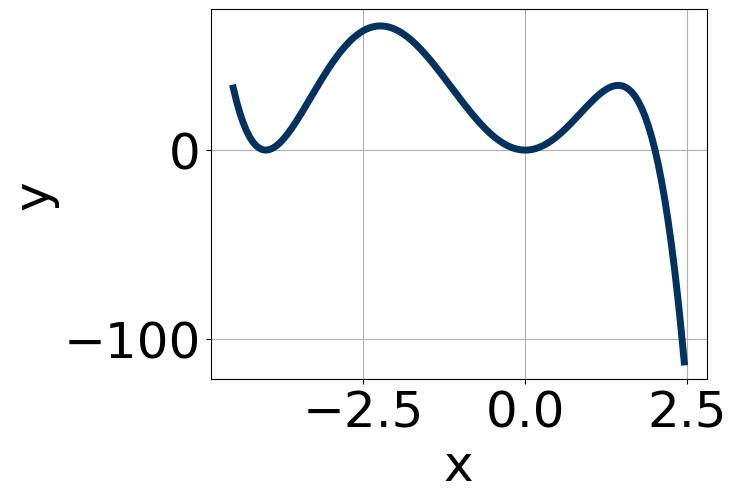
\includegraphics[width=0.5\textwidth]{../Figures/polyGraphToFunctionCopyC.png}
\end{center}



The solution is \( 11x^{11} (x + 4)^{7} (x + 1)^{5} \), which is option A.\begin{enumerate}[label=\Alph*.]
\item \( 11x^{11} (x + 4)^{7} (x + 1)^{5} \)

* This is the correct option.
\item \( 17x^{6} (x + 4)^{4} (x + 1)^{9} \)

The factors $0$ and $-4$ have have been odd power.
\item \( 9x^{4} (x + 4)^{7} (x + 1)^{7} \)

The factor $0$ should have been an odd power.
\item \( -15x^{6} (x + 4)^{7} (x + 1)^{11} \)

The factor $x$ should have an odd power and the leading coefficient should be the opposite sign.
\item \( -9x^{9} (x + 4)^{5} (x + 1)^{5} \)

This corresponds to the leading coefficient being the opposite value than it should be.
\end{enumerate}

\textbf{General Comment:} General Comments: Draw the x-axis to determine which zeros are touching (and so have even multiplicity) or cross (and have odd multiplicity).
}
\litem{
Which of the following equations \textit{could} be of the graph presented below?

\begin{center}
    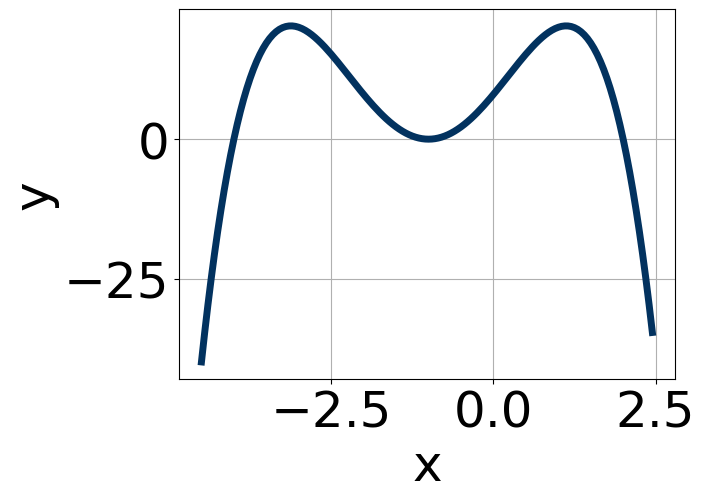
\includegraphics[width=0.5\textwidth]{../Figures/polyGraphToFunctionC.png}
\end{center}



The solution is \( -19(x + 1)^{4} (x + 2)^{7} (x - 3)^{7} \), which is option E.\begin{enumerate}[label=\Alph*.]
\item \( -13(x + 1)^{8} (x + 2)^{10} (x - 3)^{9} \)

The factor $(x + 2)$ should have an odd power.
\item \( 11(x + 1)^{10} (x + 2)^{9} (x - 3)^{8} \)

The factor $(x - 3)$ should have an odd power and the leading coefficient should be the opposite sign.
\item \( 8(x + 1)^{6} (x + 2)^{7} (x - 3)^{5} \)

This corresponds to the leading coefficient being the opposite value than it should be.
\item \( -20(x + 1)^{7} (x + 2)^{4} (x - 3)^{5} \)

The factor $-1$ should have an even power and the factor $-2$ should have an odd power.
\item \( -19(x + 1)^{4} (x + 2)^{7} (x - 3)^{7} \)

* This is the correct option.
\end{enumerate}

\textbf{General Comment:} General Comments: Draw the x-axis to determine which zeros are touching (and so have even multiplicity) or cross (and have odd multiplicity).
}
\litem{
Describe the zero behavior of the zero $x = -8$ of the polynomial below.
\[ f(x) = 4(x - 8)^{9}(x + 8)^{10}(x + 6)^{7}(x - 6)^{10} \]
The solution is the graph below, which is option C.
\begin{center}
    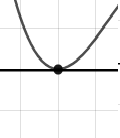
\includegraphics[width=0.3\textwidth]{../Figures/polyZeroBehaviorCC.png}
\end{center}\begin{enumerate}[label=\Alph*.]
\begin{multicols}{2}
\item 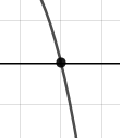
\includegraphics[width = 0.3\textwidth]{../Figures/polyZeroBehaviorAC.png}
\item 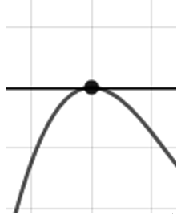
\includegraphics[width = 0.3\textwidth]{../Figures/polyZeroBehaviorBC.png}
\item 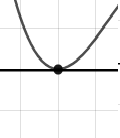
\includegraphics[width = 0.3\textwidth]{../Figures/polyZeroBehaviorCC.png}
\item 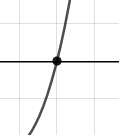
\includegraphics[width = 0.3\textwidth]{../Figures/polyZeroBehaviorDC.png}
\end{multicols}\item None of the above.\end{enumerate}
\textbf{General Comment:} You will need to sketch the entire graph, then zoom in on the zero the question asks about.
}
\litem{
Describe the end behavior of the polynomial below.
\[ f(x) = 2(x + 2)^{5}(x - 2)^{10}(x - 9)^{2}(x + 9)^{2} \]
The solution is the graph below, which is option D.
\begin{center}
    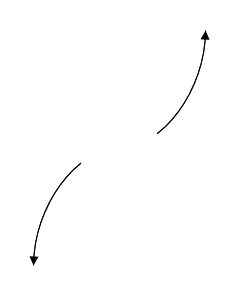
\includegraphics[width=0.3\textwidth]{../Figures/polyEndBehaviorDC.png}
\end{center}\begin{enumerate}[label=\Alph*.]
\begin{multicols}{2}
\item 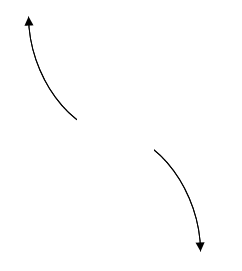
\includegraphics[width = 0.3\textwidth]{../Figures/polyEndBehaviorAC.png}
\item 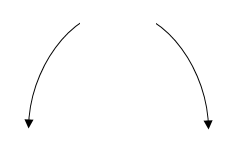
\includegraphics[width = 0.3\textwidth]{../Figures/polyEndBehaviorBC.png}
\item 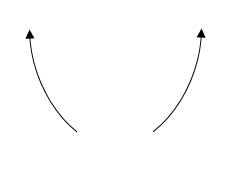
\includegraphics[width = 0.3\textwidth]{../Figures/polyEndBehaviorCC.png}
\item 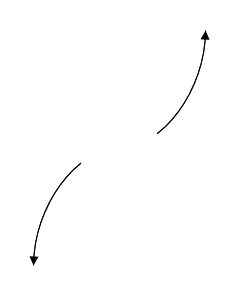
\includegraphics[width = 0.3\textwidth]{../Figures/polyEndBehaviorDC.png}
\end{multicols}\item None of the above.\end{enumerate}
\textbf{General Comment:} Remember that end behavior is determined by the leading coefficient AND whether the \textbf{sum} of the multiplicities is positive or negative.
}
\litem{
Construct the lowest-degree polynomial given the zeros below. Then, choose the intervals that contain the coefficients of the polynomial in the form $ax^3+bx^2+cx+d$.
\[ \frac{-7}{3}, -6, \text{ and } \frac{5}{4} \]
The solution is \( 12x^{3} +85 x^{2} +43 x -210 \), which is option D.\begin{enumerate}[label=\Alph*.]
\item \( a \in [7, 13], b \in [-121, -109], c \in [289, 294], \text{ and } d \in [-211, -202] \)

$12x^{3} -115 x^{2} +293 x -210$, which corresponds to multiplying out $(3x + 3)(x + 1)(4x -4)$.
\item \( a \in [7, 13], b \in [85, 94], c \in [34, 46], \text{ and } d \in [209, 218] \)

$12x^{3} +85 x^{2} +43 x + 210$, which corresponds to multiplying everything correctly except the constant term.
\item \( a \in [7, 13], b \in [-85, -83], c \in [34, 46], \text{ and } d \in [209, 218] \)

$12x^{3} -85 x^{2} +43 x + 210$, which corresponds to multiplying out $(3x -7)(x -6)(4x + 5)$.
\item \( a \in [7, 13], b \in [85, 94], c \in [34, 46], \text{ and } d \in [-211, -202] \)

* $12x^{3} +85 x^{2} +43 x -210$, which is the correct option.
\item \( a \in [7, 13], b \in [27, 37], c \in [-225, -220], \text{ and } d \in [209, 218] \)

$12x^{3} +29 x^{2} -223 x + 210$, which corresponds to multiplying out $(3x + 3)(x -1)(4x -4)$.
\end{enumerate}

\textbf{General Comment:} To construct the lowest-degree polynomial, you want to multiply out $(3x + 7)(x + 6)(4x -5)$
}
\litem{
Construct the lowest-degree polynomial given the zeros below. Then, choose the intervals that contain the coefficients of the polynomial in the form $ax^3+bx^2+cx+d$.
\[ \frac{-7}{3}, \frac{-5}{2}, \text{ and } -5 \]
The solution is \( 6x^{3} +59 x^{2} +180 x + 175 \), which is option E.\begin{enumerate}[label=\Alph*.]
\item \( a \in [3, 13], b \in [-2, 3], c \in [-114, -105], \text{ and } d \in [172, 177] \)

$6x^{3} + x^{2} -110 x + 175$, which corresponds to multiplying out $(3x + 3)(2x + 2)(x -1)$.
\item \( a \in [3, 13], b \in [-61, -58], c \in [176, 187], \text{ and } d \in [-181, -166] \)

$6x^{3} -59 x^{2} +180 x -175$, which corresponds to multiplying out $(3x -7)(2x -5)(x -5)$.
\item \( a \in [3, 13], b \in [29, 32], c \in [-38, -26], \text{ and } d \in [-181, -166] \)

$6x^{3} +31 x^{2} -30 x -175$, which corresponds to multiplying out $(3x + 3)(2x -2)(x -1)$.
\item \( a \in [3, 13], b \in [53, 69], c \in [176, 187], \text{ and } d \in [-181, -166] \)

$6x^{3} +59 x^{2} +180 x -175$, which corresponds to multiplying everything correctly except the constant term.
\item \( a \in [3, 13], b \in [53, 69], c \in [176, 187], \text{ and } d \in [172, 177] \)

* $6x^{3} +59 x^{2} +180 x + 175$, which is the correct option.
\end{enumerate}

\textbf{General Comment:} To construct the lowest-degree polynomial, you want to multiply out $(3x + 7)(2x + 5)(x + 5)$
}
\litem{
Construct the lowest-degree polynomial given the zeros below. Then, choose the intervals that contain the coefficients of the polynomial in the form $x^3+bx^2+cx+d$.
\[ 5 - 3 i \text{ and } 3 \]
The solution is \( x^{3} -13 x^{2} +64 x -102 \), which is option A.\begin{enumerate}[label=\Alph*.]
\item \( b \in [-16, -10], c \in [56, 67], \text{ and } d \in [-110, -98] \)

* $x^{3} -13 x^{2} +64 x -102$, which is the correct option.
\item \( b \in [7, 16], c \in [56, 67], \text{ and } d \in [99, 103] \)

$x^{3} +13 x^{2} +64 x + 102$, which corresponds to multiplying out $(x-(5 - 3 i))(x-(5 + 3 i))(x + 3)$.
\item \( b \in [-1, 2], c \in [-14, -7], \text{ and } d \in [12, 18] \)

$x^{3} + x^{2} -8 x + 15$, which corresponds to multiplying out $(x -5)(x -3)$.
\item \( b \in [-1, 2], c \in [0, 8], \text{ and } d \in [-10, -6] \)

$x^{3} + x^{2} -9$, which corresponds to multiplying out $(x + 3)(x -3)$.
\item \( \text{None of the above.} \)

This corresponds to making an unanticipated error or not understanding how to use nonreal complex numbers to create the lowest-degree polynomial. If you chose this and are not sure what you did wrong, please contact the coordinator for help.
\end{enumerate}

\textbf{General Comment:} Remember that the conjugate of $a+bi$ is $a-bi$. Since these zeros always come in pairs, we need to multiply out $(x-(5 - 3 i))(x-(5 + 3 i))(x-(3))$.
}
\litem{
Describe the end behavior of the polynomial below.
\[ f(x) = 5(x + 4)^{5}(x - 4)^{8}(x + 3)^{2}(x - 3)^{3} \]
The solution is the graph below, which is option C.
\begin{center}
    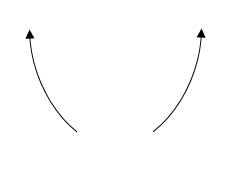
\includegraphics[width=0.3\textwidth]{../Figures/polyEndBehaviorCopyCC.png}
\end{center}\begin{enumerate}[label=\Alph*.]
\begin{multicols}{2}
\item 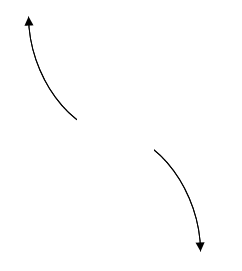
\includegraphics[width = 0.3\textwidth]{../Figures/polyEndBehaviorCopyAC.png}
\item 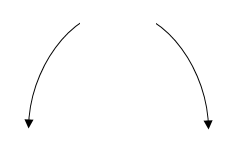
\includegraphics[width = 0.3\textwidth]{../Figures/polyEndBehaviorCopyBC.png}
\item 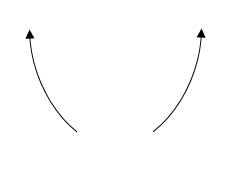
\includegraphics[width = 0.3\textwidth]{../Figures/polyEndBehaviorCopyCC.png}
\item 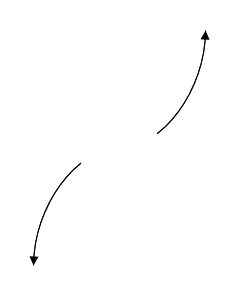
\includegraphics[width = 0.3\textwidth]{../Figures/polyEndBehaviorCopyDC.png}
\end{multicols}\item None of the above.\end{enumerate}
\textbf{General Comment:} Remember that end behavior is determined by the leading coefficient AND whether the \textbf{sum} of the multiplicities is positive or negative.
}
\litem{
Describe the zero behavior of the zero $x = 8$ of the polynomial below.
\[ f(x) = -7(x + 5)^{12}(x - 5)^{8}(x + 8)^{12}(x - 8)^{9} \]
The solution is the graph below, which is option A.
\begin{center}
    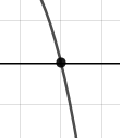
\includegraphics[width=0.3\textwidth]{../Figures/polyZeroBehaviorCopyAC.png}
\end{center}\begin{enumerate}[label=\Alph*.]
\begin{multicols}{2}
\item 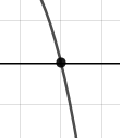
\includegraphics[width = 0.3\textwidth]{../Figures/polyZeroBehaviorCopyAC.png}
\item 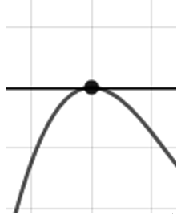
\includegraphics[width = 0.3\textwidth]{../Figures/polyZeroBehaviorCopyBC.png}
\item 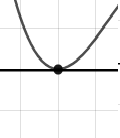
\includegraphics[width = 0.3\textwidth]{../Figures/polyZeroBehaviorCopyCC.png}
\item 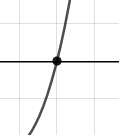
\includegraphics[width = 0.3\textwidth]{../Figures/polyZeroBehaviorCopyDC.png}
\end{multicols}\item None of the above.\end{enumerate}
\textbf{General Comment:} You will need to sketch the entire graph, then zoom in on the zero the question asks about.
}
\litem{
Construct the lowest-degree polynomial given the zeros below. Then, choose the intervals that contain the coefficients of the polynomial in the form $x^3+bx^2+cx+d$.
\[ 4 - 2 i \text{ and } -4 \]
The solution is \( x^{3} -4 x^{2} -12 x + 80 \), which is option D.\begin{enumerate}[label=\Alph*.]
\item \( b \in [-3, 3.2], c \in [-4, 5], \text{ and } d \in [-21, -7] \)

$x^{3} + x^{2} -16$, which corresponds to multiplying out $(x -4)(x + 4)$.
\item \( b \in [1.5, 4.4], c \in [-12, -8], \text{ and } d \in [-82, -75] \)

$x^{3} +4 x^{2} -12 x -80$, which corresponds to multiplying out $(x-(4 - 2 i))(x-(4 + 2 i))(x -4)$.
\item \( b \in [-3, 3.2], c \in [1, 8], \text{ and } d \in [6, 13] \)

$x^{3} + x^{2} +6 x + 8$, which corresponds to multiplying out $(x + 2)(x + 4)$.
\item \( b \in [-5.7, -2.5], c \in [-12, -8], \text{ and } d \in [80, 83] \)

* $x^{3} -4 x^{2} -12 x + 80$, which is the correct option.
\item \( \text{None of the above.} \)

This corresponds to making an unanticipated error or not understanding how to use nonreal complex numbers to create the lowest-degree polynomial. If you chose this and are not sure what you did wrong, please contact the coordinator for help.
\end{enumerate}

\textbf{General Comment:} Remember that the conjugate of $a+bi$ is $a-bi$. Since these zeros always come in pairs, we need to multiply out $(x-(4 - 2 i))(x-(4 + 2 i))(x-(-4))$.
}
\end{enumerate}

\end{document}